\documentclass[conference]{IEEEtran}
\IEEEoverridecommandlockouts
% The preceding line is only needed to identify funding in the first footnote. If that is unneeded, please comment it out.
\usepackage{url}
\usepackage{cite}
\usepackage{amsmath,amssymb,amsfonts}
\usepackage{algorithmic}
\usepackage{graphicx}
\usepackage{placeins}
\usepackage{textcomp}
\usepackage{xcolor}
\usepackage{fancyhdr}
\usepackage{subfigure} 
\usepackage{float} 
\usepackage{caption}
\usepackage{hyperref}
\usepackage{url}

\def\BibTeX{{\rm B\kern-.05em{\sc i\kern-.025em b}\kern-.08em
    T\kern-.1667em\lower.7ex\hbox{E}\kern-.125emX}}
    
% ANCS'19 Conference Name %%%%%%%%%%%%%%%%%%%%%%%%%%%%%%%%%%%%%%%%%%%%%%%%%%%%%%%%%%%%%%%%
\chead{\rmfamily\fontsize{9}{30}\selectfont 
2025 Data Mining en Ciencia y Tecnología - Maestría en data mining FCEN UBA}
\renewcommand{\headrulewidth}{0pt}
%%%%%%%%%%%%%%%%%%%%%%%%%%%%%%%%%%%%%%%%%%%%%%%%%%%%%%%%%%%%%%%%%%%%%%%%%%%%%%%%%%%%%%%%%%

% ANCS'19 Copyright Notice %%%%%%%%%%%%%%%%%%%%%%%%%%%%%%%%%%%%%%%%%%%%%%%%%%%%%%%%%%%%%%%%%%%%%%%%%%%%%%%%%%%%%%%%%%%%%%%%%
% Note: use the copyright text that matches your requirements.
%
% 1. For papers in which all authors are employed by the US government, the copyright notice is: 
%\cfoot{\rmfamily\fontsize{9}{0}\selectfont U.S. Government work not protected by U.S. copyright}
%
% 2. For papers in which all authors are employed by a Crown government (UK, Canada, and Australia), the copyright notice is: 
%\cfoot{\rmfamily\fontsize{9}{0}\selectfont 978-1-7281-4387-3/19/\$31.00~\copyright~2019 Crown}
%
% 3. For papers in which all authors are employed by the European Union, the copyright notice is:
%\cfoot{\rmfamily\fontsize{9}{0}\selectfont 978-1-7281-4387-3/19/\$31.00~\copyright~2019 European Union}
%
% 4. For all other papers the copyright notice is:
\cfoot{}
%%%%%%%%%%%%%%%%%%%%%%%%%%%%%%%%%%%%%%%%%%%%%%%%%%%%%%%%%%%%%%%%%%%%%%%%%%%%%%%%%%%%%%%%%%%%%%%%%%%%%%%%%%%%%%%%%%%%%%%%%%%%%

\begin{document}

\title{Una exploración sobre la robustez en redes humanas\\
{\footnotesize \textsuperscript{}}
}

\author{\IEEEauthorblockN{Serena Dituro}
\IEEEauthorblockA{\textit{Universidad Favaloro} \\
serenadituro@gmail.com}
\and
\IEEEauthorblockN{Lucas Chicco}
\IEEEauthorblockA{\textit{FRBA - UTN} \\
lchicco94@gmail.com}
\and
\IEEEauthorblockN{Manuel Moreira}
\IEEEauthorblockA{\textit{FFyL - UBA} \\
manuelmoreira.ar@gmail.com}
\and
\IEEEauthorblockN{Joaquín Kalmbach}
\IEEEauthorblockA{\textit{FA - UBA} \\
kalmbach.jr@gmail.com}
}

\maketitle
\thispagestyle{fancy}

\begin{abstract}
La resiliencia de las redes humanas es un aspecto clave en el estudio de grafos reales. Motivados por el interés en comprender el comportamiento humano en comunidad, analizamos y comparamos dos redes: la de co-ocurrencias de personajes en 'Les Miserables' y la de intercambios de correos electrónicos en una institución europea. Nos propusimos evaluar su estructura y robustez, aplicando métricas topológicas como grado, clustering y centralidades, y comparándolas con prototipos conocidos como redes aleatorias, de mundo pequeño y libres de escala.

Además del análisis estructural, exploramos la formación de comunidades, observando agrupamientos más definidos en la red literaria y una organización más dispersa en la red de correos. A través de simulaciones de ataques aleatorios y dirigidos, observamos que la red de 'Les Miserables' colapsa rápidamente al eliminar nodos centrales, lo cual brinda indicios de una red libre de escala, mientras que la red de Emails logra sostener su conectividad por más tiempo, asemejándola a una red de mundos pequeños. 

Aunque las variables topológicas indicaron distintos prototipos equivalentes, los ataques dirigidos proporcionaron una señal más clara del modelo al que mejor se adapta cada red.
\end{abstract}



\begin{IEEEkeywords}
redes, grafos, robustez, centralidad, comunidades
\end{IEEEkeywords}

\section{\textbf{Introducción}}

En el presente trabajo, se realiza la selección de dos datasets de interés, que tienen algunos puntos de coincidencia pero son muy diferentes entre sí, con la motivación particular de investigar sobre la resiliencia de las mismas ante perturbaciones. 

A continuación se realiza una breve descripción de las redes seleccionadas:
Por un lado, la red de Les Misèrables es una red pequeña de 77 nodos y 254 enlaces que está construida a partir de la copresencia de personajes en los capítulos de la novela, se trata de una red pesada en la cual el peso de cada enlace representa la frecuencia de co-ocurrencia, al solo medir co-ocurrencia los enlaces son no-dirigidos. Es una red muy utilizada en el ámbito de la enseñanza de análisis redes, por lo que pueden encontrarse numerosas publicaciones que utilizan esta red como insumo, como el trabajo de  Mouschoutzi\cite{mouschoutzi2024}, quien estudió esta red enfocándose en medidas de centralidad. 
Por su parte, la red de Emails-EU también es una red muy famosa en el ámbito de análisis de redes y cuenta con numerosas publicaciones que la utilizan como fuente \cite{nr}. La misma está construida a partir del intercambio de emails entre integrantes de una institución de investigación de la unión europea, los lazos no tienen peso ni dirección solamente dan cuenta de que existió un intercambio de emails entre dos integrantes que están representados como nodos.

En base a las publicaciones mencionadas, formulamos la hipótesis que sostiene que la red de Emails será más resiliente a fallas nodales que la red de Les Misèrables, debido a su tamaño, grado medio y una posible distribución de conectividad más homogénea o distribuida. En el presente trabajo, buscaremos responder a la siguiente pregunta: ¿Cuál de las redes muestra mayor resiliencia estructural ante la remoción de nodos críticos, y cómo se compara esa resiliencia con la de una red aleatoria del mismo tamaño?

A partir de dicha pregunta de investigación, nos proponemos abordar los principales objetivos del presente trabajo:

\begin{enumerate}
    \item Calcular variables topológicas que describan el comportamiento de las redes seleccionadas, así como efectuar la comparación de las mismas con modelos prototipos equivalentes que permitan sacar conclusiones sobre una mayor o menor aproximación a modelos de redes extensamente conocidos.
    
    \item Realizar el análisis de centralidad de los nodos.
    
    \item Efectuar el análisis de robustez de los grafos, cuyos resultados permitan responder a la pregunta de investigación que motiva el desarrollo del presente trabajo.
    
    \item Detectar comunidades en los grafos.
\end{enumerate}


\vspace{15pt}

\section{Materiales y Métodos}

Los análisis de redes se realizaron utilizando los conceptos y algoritmos descritos en el libro Network Science de Albert-László Barabási\cite{barabasi2016}(2016). Las implementaciones de los algoritmos de detección de comunidades (Louvain y Girvan-Newman), así como las métricas de centralidad y robustez, se basaron en la librería NetworkX (Hagberg et al., 2008) de Python \cite{networkx2008}. Esta librería proporciona una plataforma flexible y eficiente para el análisis y la manipulación de grafos, permitiendo la aplicación de los métodos descritos por Barabási a las redes estudiadas.

\vspace{10pt}

\subsection{{Métricas de redes}}
En principio, se calcularon diferentes variables topológicas de las redes seleccionadas, entre las que se destacan el coeficiente de clustering, la densidad, la distancia media, la eficiencia global, etc. Luego, se manipularon las redes con el objetivo de garantizar que sean grafos no dirigidos ni pesados; y en el caso de que sea una red no conectada, se trabajó con la componente gigante. A partir de entonces, se obtuvieron prototipos equivalentes de modelos de redes extensamente conocidos, como el de Erdos-Renyi (Aleatorio), Watts-Strogatz (Mundo pequeño), Barabasi-Albert (Libre de escala) y Holme-Kim. Finalmente, se realizaron comparaciones de las distribuciones de grado en términos del coeficiente de clustering promedio, la distancia media promedio y el grado promedio, lo que permitió no sólo un entendimiento general de las redes elegidas, sino también adentrarnos en un análisis más profundo de los aspectos más interesantes de cada una.
\subsection{Centralidad}
Se binarizó la red de 'Les Miserables' para que la comparación de centralidades parta de un criterio en común.
Se calculó la Centralidad de grado y la Centralidad de Intermediación para ambas redes. 
Utilizando matplotlib para graficar las redes y ajustando el tamaño de los nodos según su nivel de centralidad. Además se eligió la paleta de color coolwarm, la cual pinta de azul los valores más bajos y de rojo los más altos. 
Se implementó spring-layout para los layouts de los grafos. Para el grafo de los mails se utilizó scale= 10, se eliminaron los labels y se dibujaron las relaciones con trazos más finos para poder visualizar mejor los Nodos. Mientras que para 'Les Miserables' no se implementó ninguna escala puntual y se mantuvieron los labels de los nodos.
\begin{enumerate}
    \item Analizamos rasgos topológicos principales
    \item Sacamos peso y autoreferencias a la red de mails y volvemos a evaluar
    \item Creamos red a partir de los departamentos de los mails y volvemos a comparar
    \item Credamos redes prototipos (al azar para analizar y comparar)
    \item Simulamos fallas/ataques y analizamos respuestas de redes (ataques al azar y dirigidos)
\end{enumerate}


\subsection{Robustez}
Para el análisis de robustez se partió de lo expuesto en centralidad donde se observaron los nodos de mayor centralidad de acuerdo a diferentes métodos. Con esto, se procedió a comparar el comportamiento de la componente gigante y de la eficiencia global de ambas redes frente a extracciones de nodos ya sea de forma aleatoria como de forma estratégica quitando nodos de alta centralidad, de modo de lograr determinar a qué tipo de prototipo se asemeja cada red y cuán resiliente es una respecto de la otra. 
\subsection{Detección de comunidades}
Para detección de comunidades trabajamos con 2 algoritmos diferentes, por un lado  Girvan-Newman, un algoritmo clásico con enfoque top-down para detección de comunidades y por el otro Louvain, un algoritmo más ágil de enfoque bottom-up.
Dado que el algoritmo de Louvain puede arrojar resultados dispares por diseño, tomamos la decisión de correr 100 iteraciones y tomar el resultado con mayor modularidad.
En el caso de 'Les Miserables' ambos algoritmos dieron resultados con modularidad fuerte un números de comunidades bajos, entre 6 y 11. Como se pueden ver en la imagen \ref{fig:curva-modularidad} la modularidad calculada mediante Girvan-Newman encuentra su pico óptimo en 11 comunidades

\begin{figure}[!h]
    \centering
    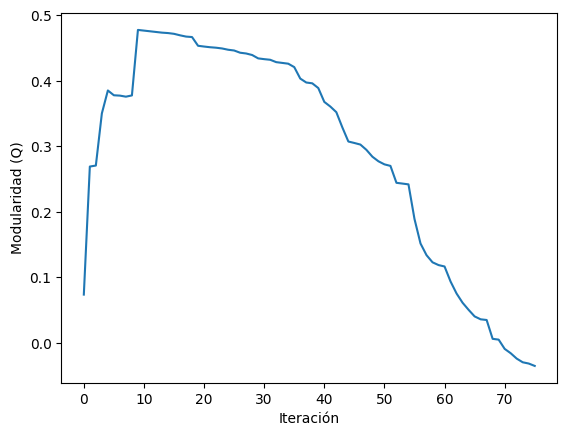
\includegraphics[width=\linewidth]{img/comu_GNlesmisModularity.png} % Remove multiplier
    \caption{Evolución de la modularidad en función de la cantidad de comunidades, Emails Girvan Newman}
    \label{fig:curva-modularidad}
\end{figure}

La red de Emails EU por su parte, mostró diferencias notables entre los dos algoritmos en cuanto a resultados y performance. Los problemas de performance fueron tan notables que hicieron imposible la repetición de los cálculos.

Respecto a la comparación entre las comunidades detectadas y las etiquetas de departamentos, utilizamos 3 métodos;
\begin{enumerate}
    \item adjusted rand score(ARS) que arrojó un valor de 0.3250
    \item normalized mutual info score (MNI) que arrojó un valor de 0.5813
    \item Una tabla de contingencia para evaluar la correlación entre departamentos y comunidades 
\end{enumerate}

\vspace{15pt}

\section{\textbf{Resultados y discusión}}

\vspace{10pt}

Al comparar ambas redes sin ningún tipo de modificación, observamos que poseen rasgos topológicos distintos. Entre sus principales diferencias se pudo ver que la red de '''Les Miserables'' es mucho menor a la de emails, a su vez está totalmente conectada mientras que la segunda no lo está. En la tabla 1 se ilustran las principales comparaciones.

\begin{table}[h]
\centering
\begin{tabular}{|l|c|c|}
\hline
\textbf{Métrica} & \textbf{Email} & \textbf{'Les Miserables'} \\
\hline
Nodos & 1005 & 77 \\
\hline
Aristas & 16706 & 254 \\
\hline
Grafo Dirigido & No & No \\
\hline
Grafo Pesado & No & Sí \\
\hline
Está Conectado & No & Sí \\
\hline
Densidad & 0.0331 & 0.0868 \\
\hline
Coef. Clustering Promedio & 0.3994 & 0.5731 \\
\hline
Eficiencia Global & 0.4043 & 0.4353 \\
\hline
Distancia Media & - & 2.6411 \\
\hline
Nº de Componentes & 20 & 1 \\
\hline
\end{tabular}
\vspace{5pt}
\caption{Comparación de propiedades básicas entre las redes Email y 'Les Miserables'.}
\label{tab:comparacion_redes}
\end{table}
\FloatBarrier
Una vez eliminados los pesos de las aristas en la red de 'Les Miserables' y seleciconado solamente el componente gigante de la red de emails, se calculó nuevamente las características generales de las redes, obteniendo lso resultados de la tabla 2.
\vspace{5pt}
\begin{table}[h]
    \centering
    \begin{tabular}{|l|c|c|}
        \hline
        \textbf{Métricas} & \textbf{Email (Comp. Gig.)} & \textbf{Les Mis. (Unweigh.)} \\
        \hline
        Nodos & 986 & 77 \\
        \hline
        Aristas & 16064 & 254 \\
        \hline
        Dirigido & No & No \\
        \hline
        Pesado & No & No \\
        \hline
        Conectado & Sí & Sí \\
        \hline
        Densidad & 0.0331 & 0.0868 \\
        \hline
        Coef. Clustering Prom. & 0.4071 & 0.5731 \\
        \hline        
        Distancia Media & 2.587 & 2.641 \\
        \hline
        Nº de Componentes & 1 & 1 \\
        \hline
    \end{tabular}
    \vspace{5pt}
    \caption{Comparación entre el componente gigante de Email y la red de 'Les Miserables' no ponderada.}
    \label{tab:comparacion_componentes}
\end{table}

\subsection{\textbf{Comparación de redes con prototipos equivalentes}}

\vspace{10pt}

Para llevar a cabo la comparación de las redes seleccionadas con sus prototipos equivalentes, se manipulan los datasets de forma tal de trabajar con grafos no dirigidos ni pesados. En particular, para el dataset de emails, se trabaja con la componente gigante, dado que se trata de un grafo no conectado.

\vspace{10pt}

En principio, se grafica la distribución de grado de las redes elegidas (Figura 2):

\begin{figure}[h]
    \centering
    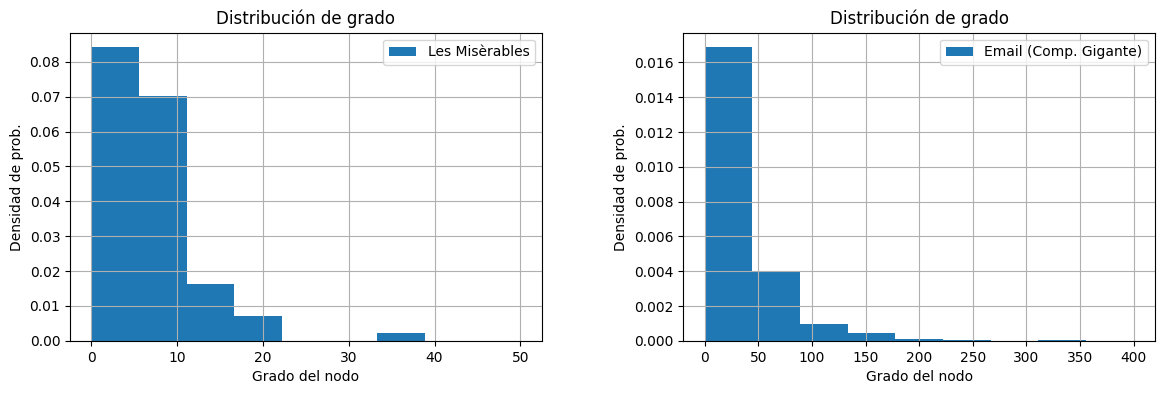
\includegraphics[width=3.5in]{img/comp-distrib_grado.png}
    \caption{Distribución de grado del grafo “Les Misèrables” y de la componente gigante de la red de Emails.}
    \label{fig:lesmis-avg_clus}
\end{figure}
\FloatBarrier

Se observa que ambos grafos se corresponden con el comportamiento típico de una red libre de escala (Barabasi-Albert), dado que la distribución sigue una ley de potencia, determinada por la existencia de una gran cantidad de nodos con pocos enlaces y un pequeño número de nodos muy conectados ("Hubs").

\vspace{10pt}

En los siguientes gráficos, se realiza la comparación entre los datasets seleccionados y sus prototipos equivalentes que se corresponden con los modelos de redes de Erdos-Renyi (Aleatorio), Watts-Strogatz (Mundo pequeño), Barabasi-Albert (Libre de escala) y Holme-Kim, en términos del coeficiente de clustering promedio, la distancia mínima media y el grado medio:

\begin{figure}[h]
    \centering
    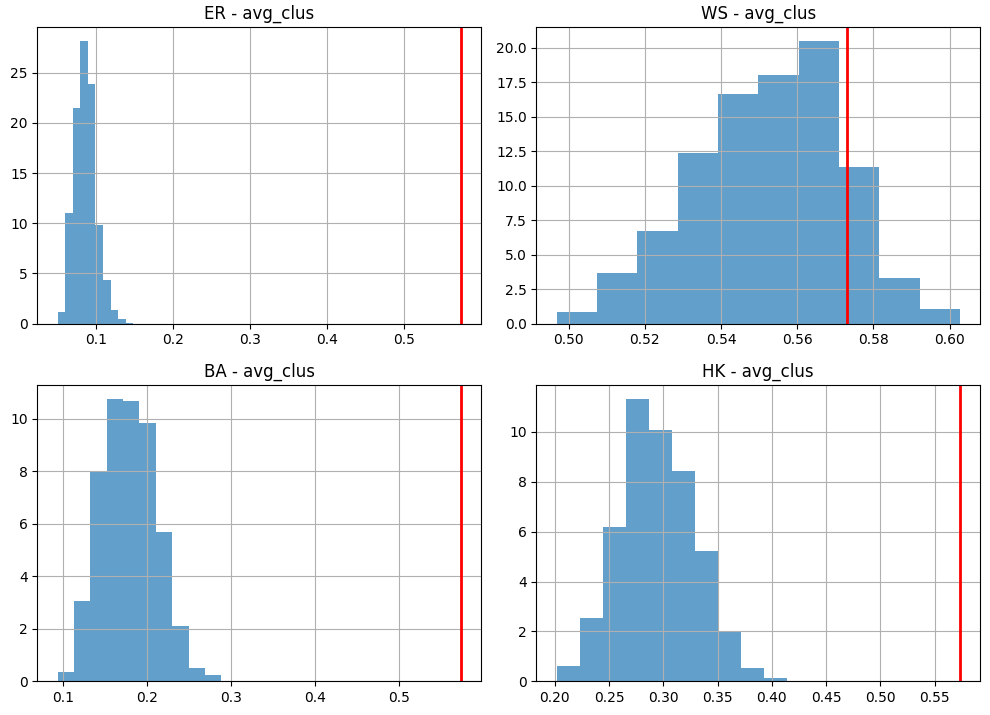
\includegraphics[width=3.5in]{img/comp-prototipos_nm_lesmis-avg_clus.png}
    \captionsetup{width=0.85\linewidth, font=small}
    \caption{Comparativa entre el grafo “Les Misèrables” (línea roja) y sus prototipos equivalentes de Erdos-Renyi (ER), Watts-Strogatz (WS), Barabasi-Albert (BA) y Holme-Kim (HK), en términos del coeficiente de clustering promedio, considerando 1000 instancias.}
    \label{fig:lesmis-avg_clus}
\end{figure}

\begin{figure}[h]
    \centering
    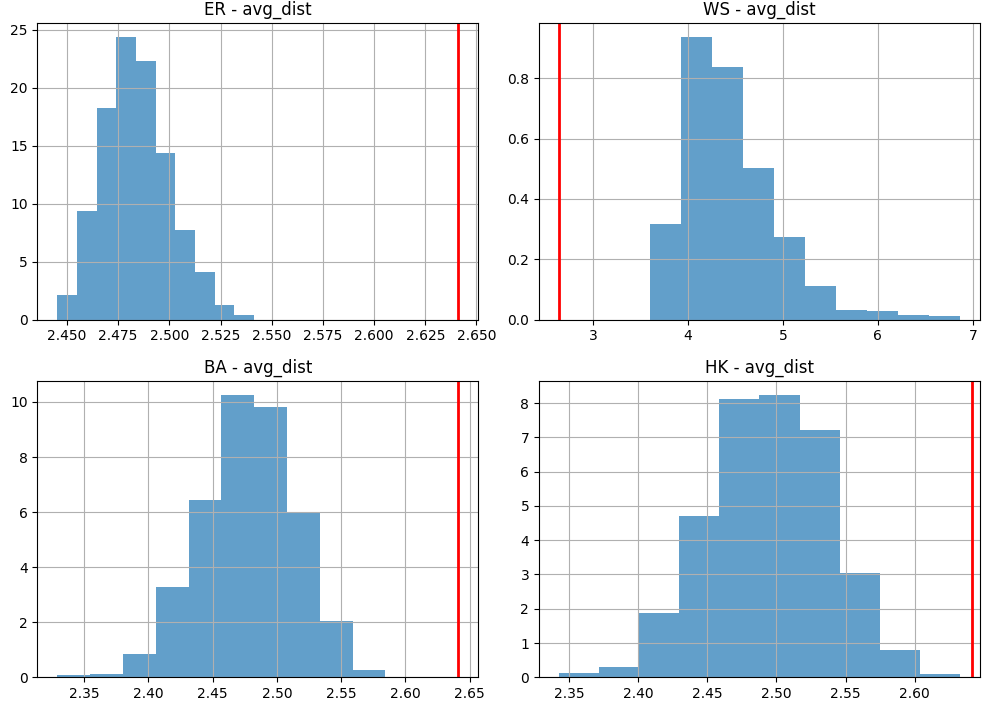
\includegraphics[width=3.5in]{img/comp-prototipos_nm_lesmis-avg_distance.png}
    \captionsetup{width=0.85\linewidth, font=small}
    \caption{Comparativa entre el grafo “Les Misèrables” (línea roja) y sus prototipos equivalentes de Erdos-Renyi (ER), Watts-Strogatz (WS), Barabasi-Albert (BA) y Holme-Kim (HK), en términos de la distancia mínima media, considerando 1000 instancias.}
    \label{fig:lesmis-avg_distance}
\end{figure}

\begin{figure}[h]
    \centering
    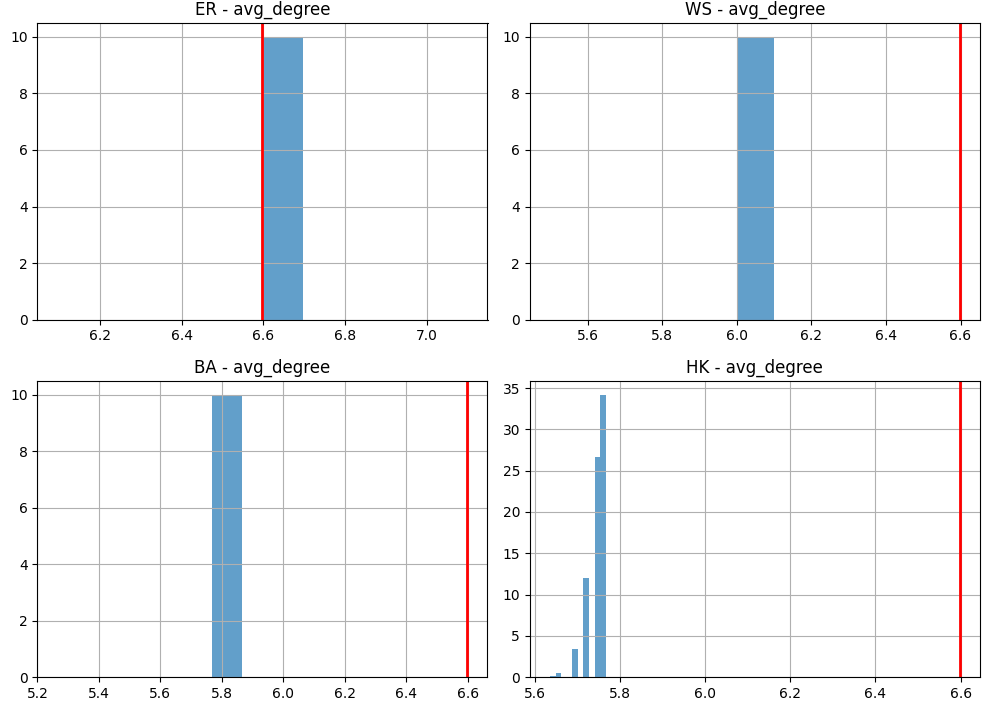
\includegraphics[width=3.5in]{img/comp-prototipos_nm_lesmis-avg_degree.png}
    \captionsetup{width=0.85\linewidth, font=small}
    \caption{Comparativa entre el grafo “Les Misèrables” (línea roja) y sus prototipos equivalentes de Erdos-Renyi (ER), Watts-Strogatz (WS), Barabasi-Albert (BA) y Holme-Kim (HK), en términos del grado medio.}
    \label{fig:lesmis-avg_degree}
\end{figure}


\FloatBarrier


Considerando la comparación de los grafos con sus respectivos prototipos equivalentes, en ambos casos se obtienen resultados semejantes en términos de los parámetros analizados. Se concluye que el modelo que mejor ajusta los coeficientes de clustering promedio (avg\_clus) es el de Watts-Strogatz (WS), asociado a números relativamente altos. Respecto a las distancias mínimas media (avg\_dist), no se observan grandes diferencias entre los modelos, ya que se mantienen en rangos relativamente razonables en torno a los valores reales. Lo mismo ocurre con los grados medio (avg\_degree), donde si bien el de Erdos-Renyi (ER) es el que mejor se ajusta, los demás modelos se encuentran próximos, si se enfatiza en la escala utilizada.

A partir del siguiente gráfico que relaciona el camino mínimo medio y el coeficiente de clustering promedio entre los grafos reales estudiados y sus prototipos equivalentes (Figura 6) se observa que el modelo WS es el que mejor se ajusta en términos del coeficiente de clustering promedio, especialmente en el grafo de "Les Misèrables", mientras que los modelos BA y ER se aproximan mejor respecto al parámetro del camino mínimo medio.

\begin{figure}[h]
    \centering
    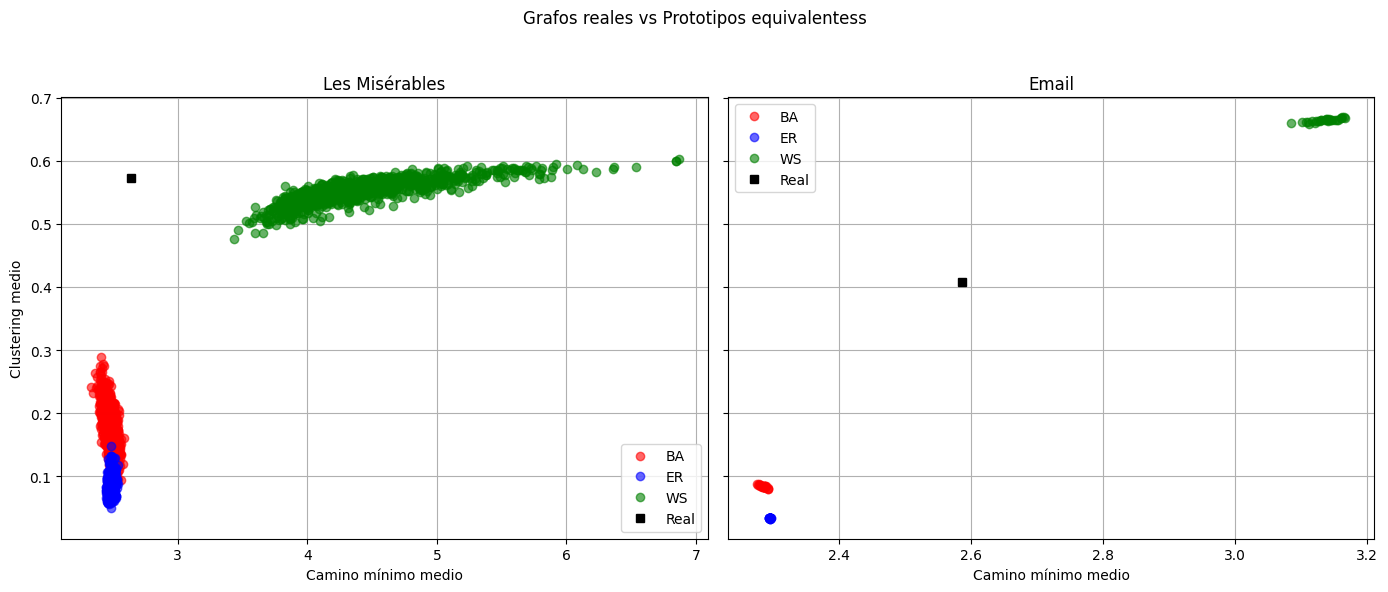
\includegraphics[width=3.5in]{img/comp-camino medio vs clust.png}
    \caption{Comparativa entre la distancia mínima media vs el coeficiente de clustering promedio del grafo de "Les Misèrables" y sus prototipos equivalentes.}
    \label{fig:emails-avg_distance}
\end{figure}

A continuación se visualiza la distribución de Powerlaw ajustada al modelo de Baravasi-Albert para ambos grafos estudiados:

\begin{figure}[h]
    \centering
    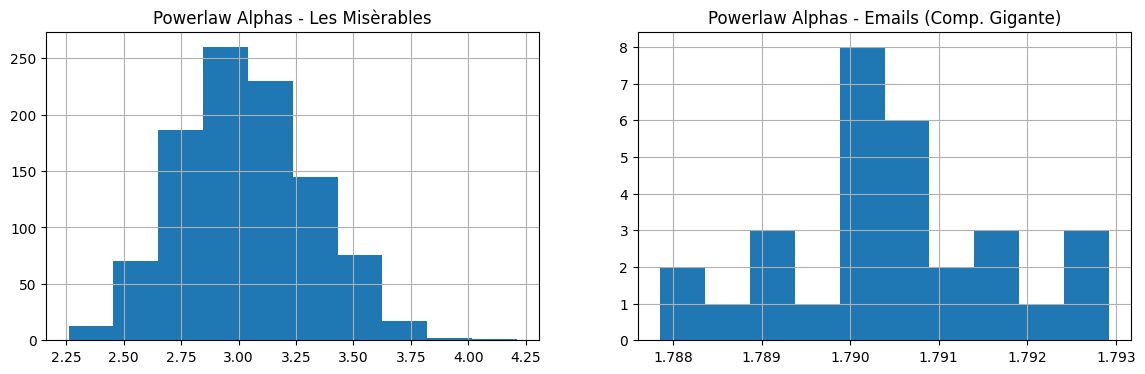
\includegraphics[width=3.5in]{img/powerlaw.png}
    \caption{Distribución de Powerlaw ajustada al modelo de Baravasi-Albert del grafo de "Les Misèrables" y de la componente gigante de la red de "Emails".}
    \label{fig:emails-avg_degree}
\end{figure}

Al igual que la Figura 2, estos gráficos determinan que ambas redes tienen una estructura libre de escala, caracterizadas por una distribución de grados que sigue una ley de potencias, con una mayoría de nodos de bajo grado y unos pocos con grado alto. En términos prácticos, esto refleja que en la red de "Les Misérables", existen personajes principales, con roles protagónicos, que interactúan con muchos otros personajes secundarios; mientras que en la red de "Emails", existen usuarios de gran experiencia, líderes y con muchos contactos que actúan de nexo entre los demás. 

%\FloatBarrier

\vspace{5pt}

\subsection{Análisis de centralidad}

\subsubsection{Emails - Componente Gigante}

En el gráfico de centralidad de grado, se puede observar que existe gran cantidad de nodos muy conectados. Lo cual indica una alta relación en general.

\begin{figure}[H]
    \centering
    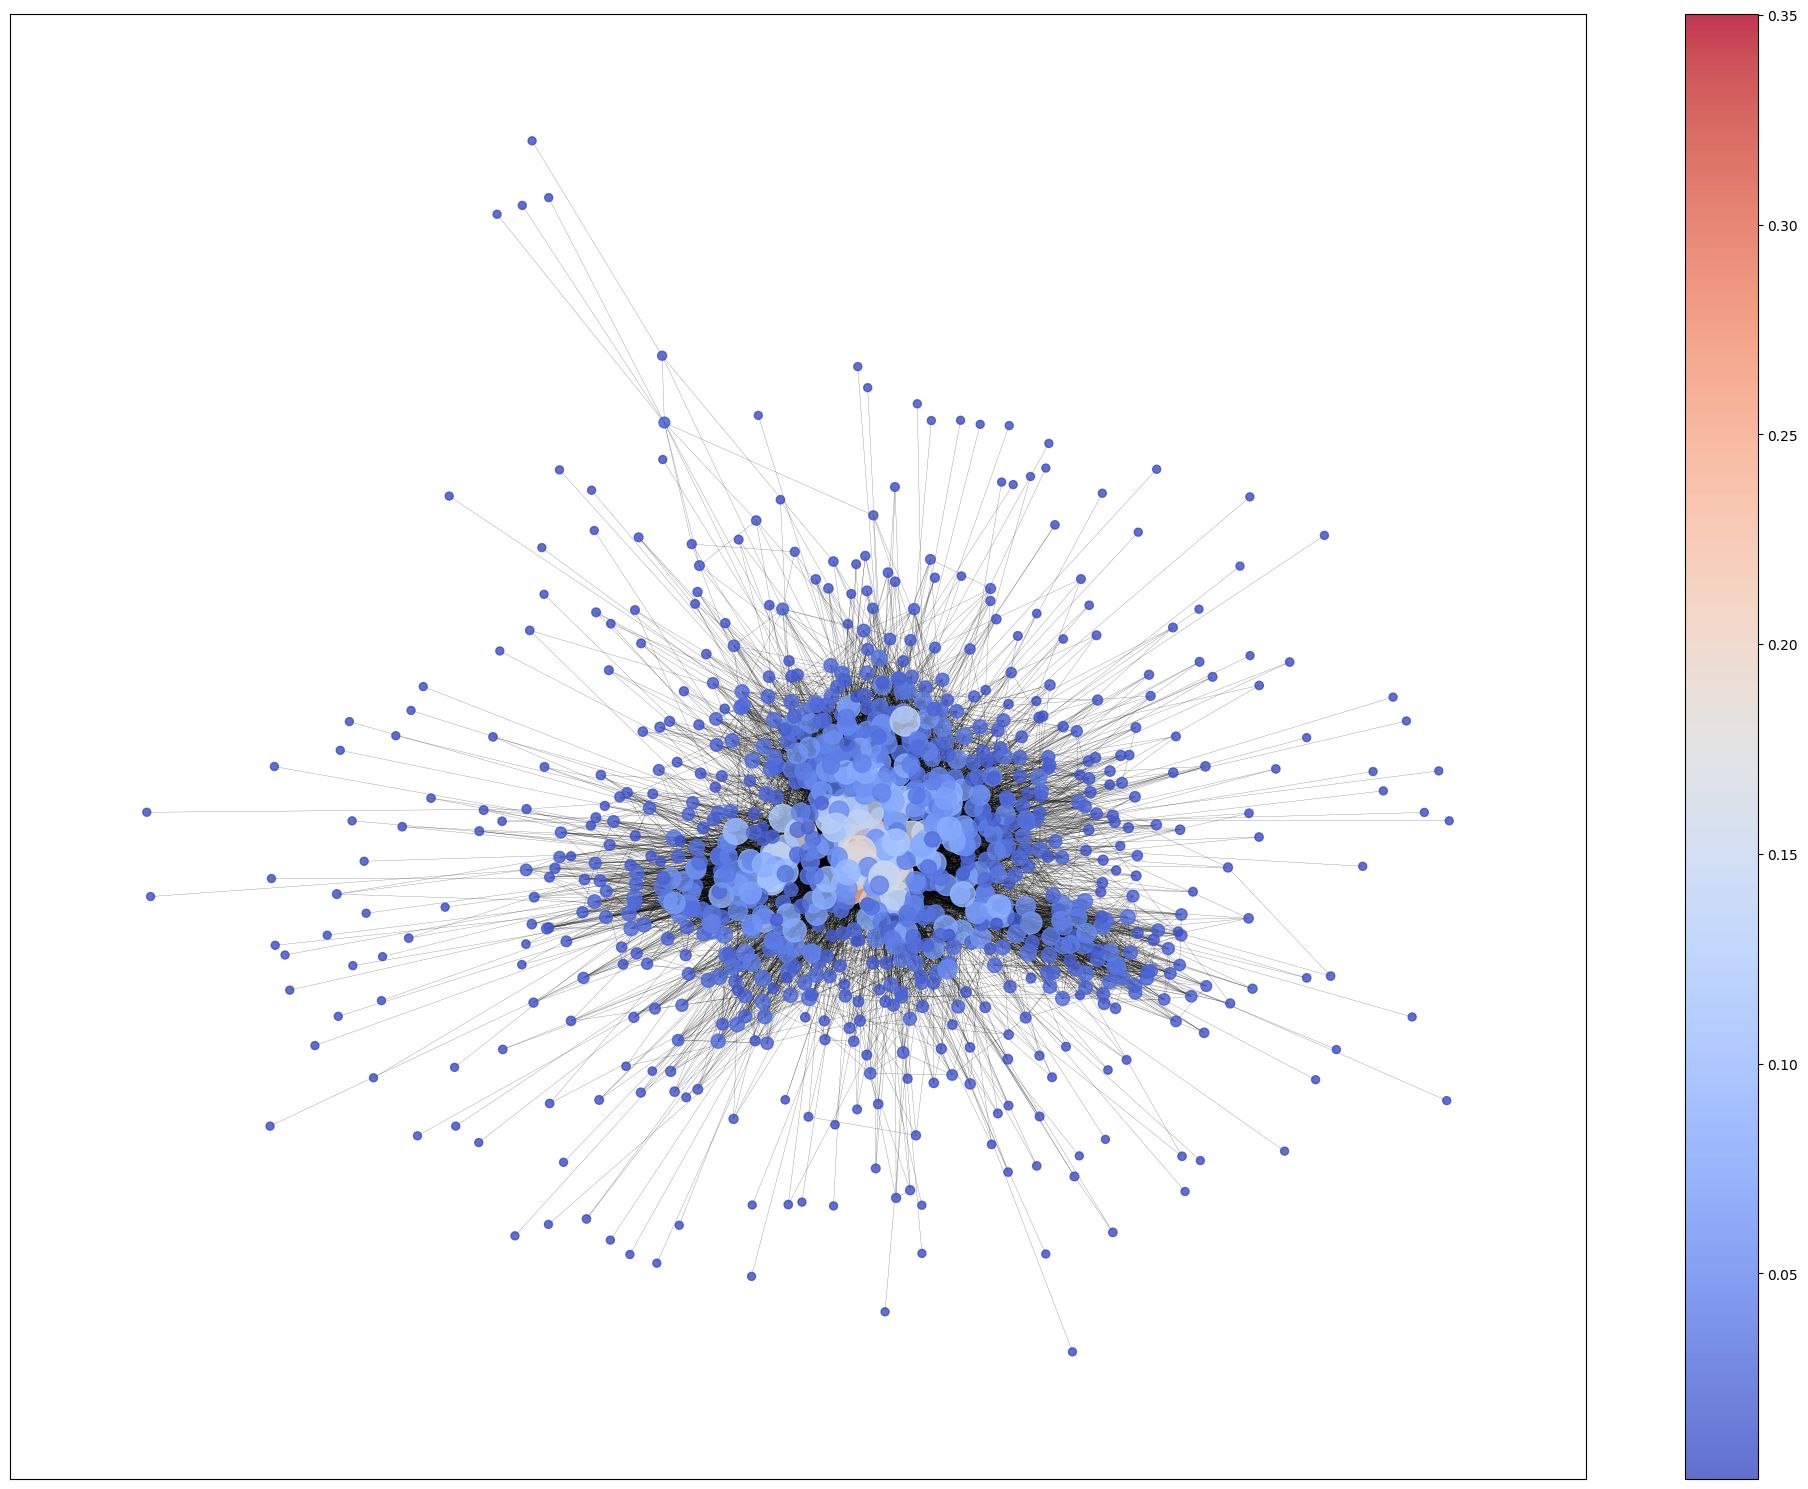
\includegraphics[width=3in]{img/centralidad_emails_degrees_sping.png}
    \caption{Centralidad de Grado - Email Componente Gigante}
    \label{fig:degree_email}
\end{figure}


Se destacan los nodos más conectados (quienes más emails enviaron o recibieron). Como se destacó anteriormente, estos nodos pueden representar a usuarios de gran experiencia, líderes y con muchos contactos .


En el gráfico de centralidad de intermediación, los nodos en general pierden centralidad, quedando muchos menos nodos como importantes. Lo que se puede observar es que los nodos con mayor centralidad en este caso también tienen alta centralidad de grado. Lo cual indica cierta correlación.

\begin{figure}[h]
    \centering
    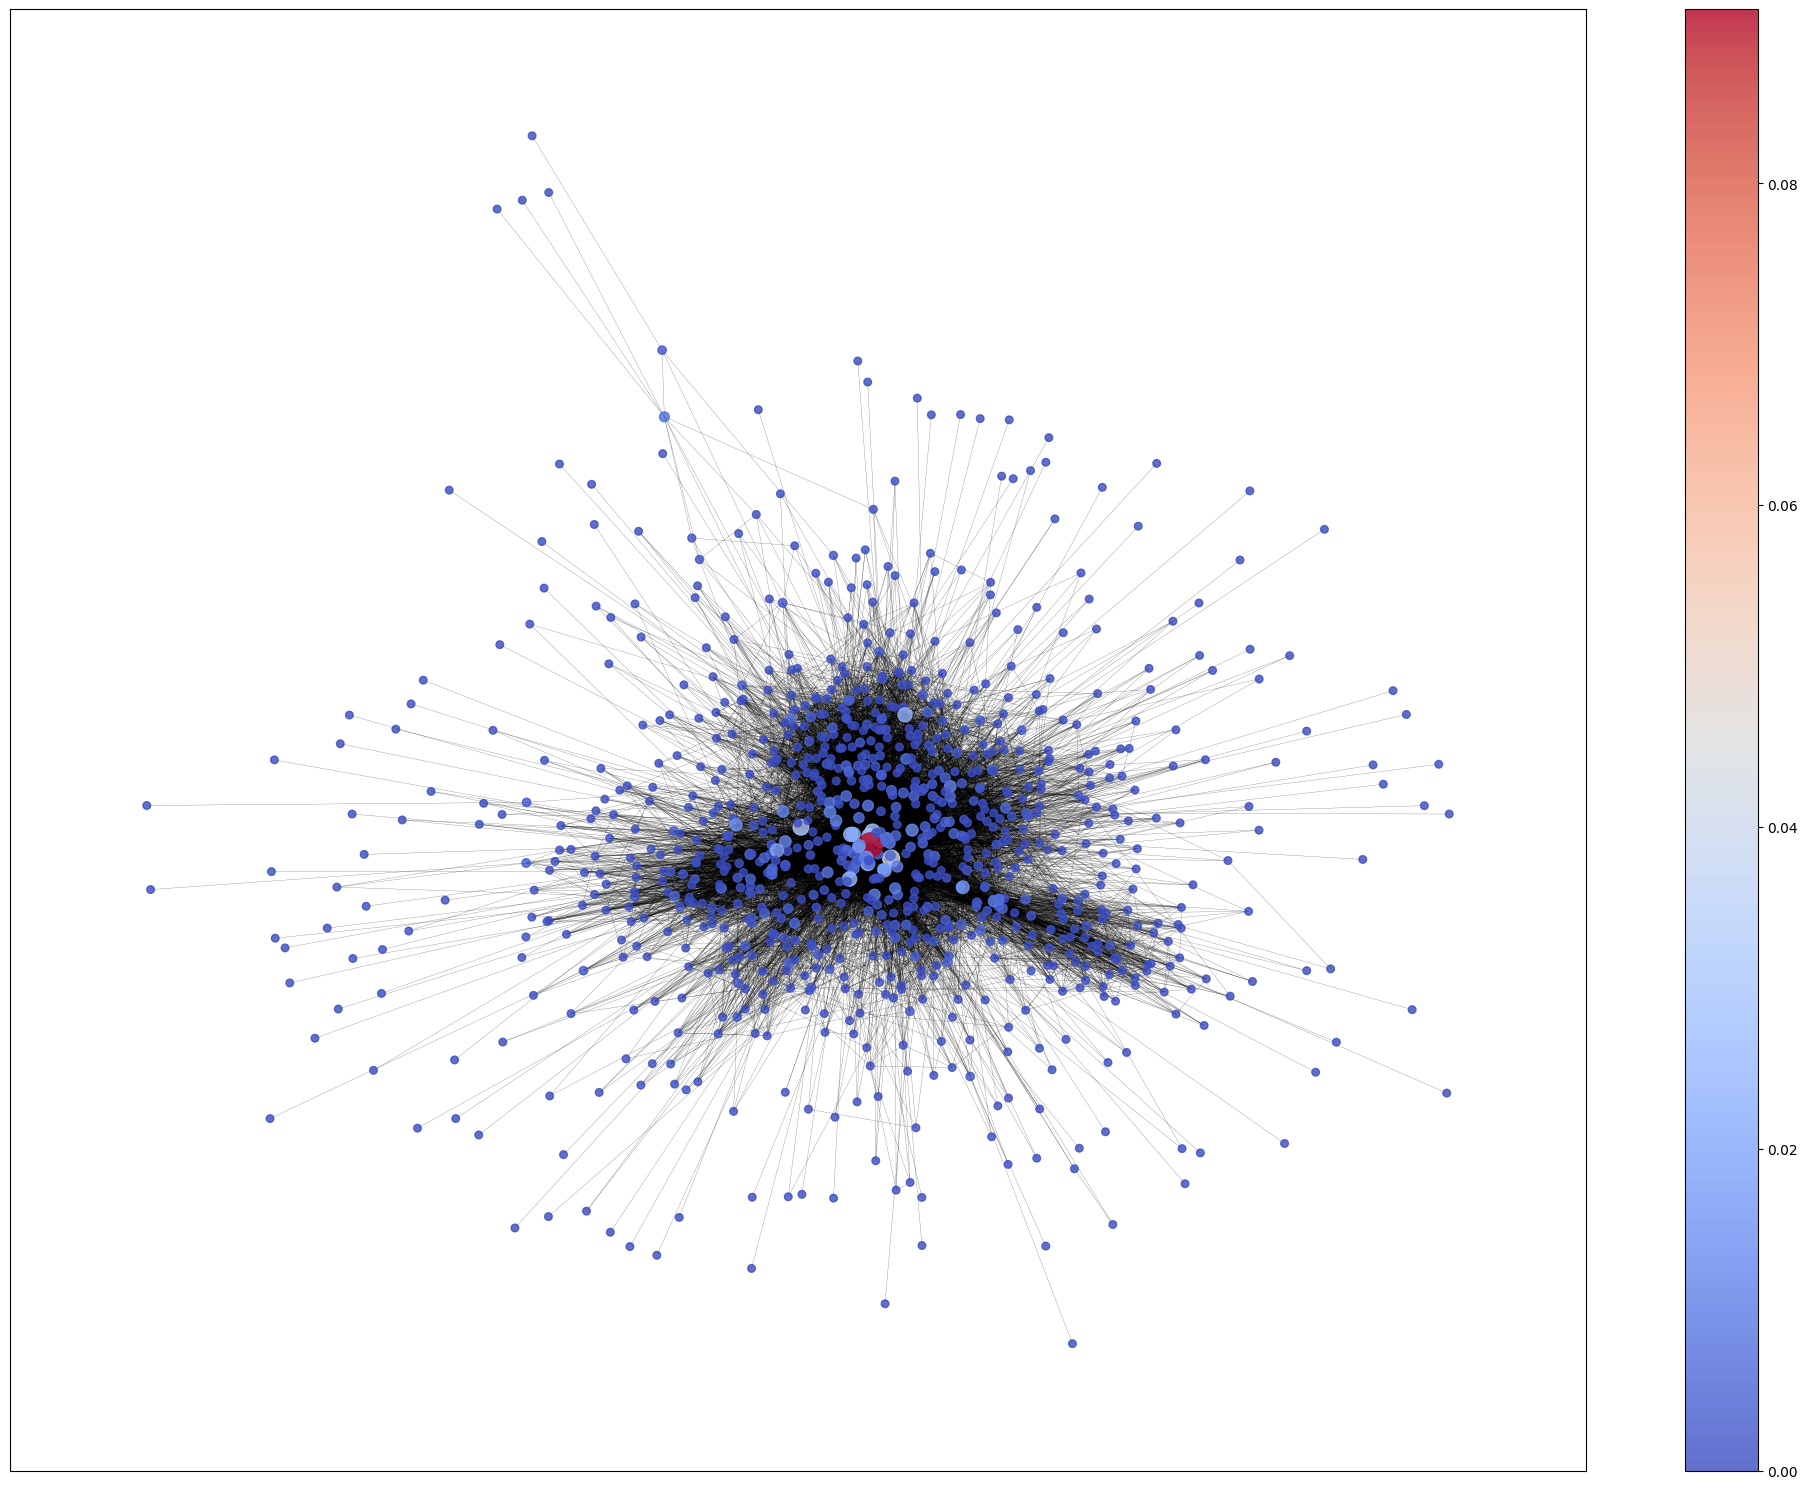
\includegraphics[width=3in]{img/centralidad_email_betweness_sping.png}
    \caption{Centralidad de intermediación - Email Componente Gigante}
    \label{fig:betweneess_email}
\end{figure}

De esta manera podríamos pensar que en general hay una alta interrelación envíos de mails entre los distintos correos. Pero el flujo de la información depende sobre todo de unos pocos. Lo cual podría explicarse como mails de comunicación entre departamentos o con roles de comunicación puntual. 

\subsubsection{'Les Miserables'}

Usando la centralidad de grado, se observa que para el grafo 'Les Miserables', el nodo 10 es el que más importancia tiene dentro de la red. Seguido por el 55, 48, 25 y 23. En esta distribución. Mientras que el 10 se vincula con todos ellos los otros cuatro se encuentran cercanos a varios nodos. 

\begin{figure}[h]
    \centering
    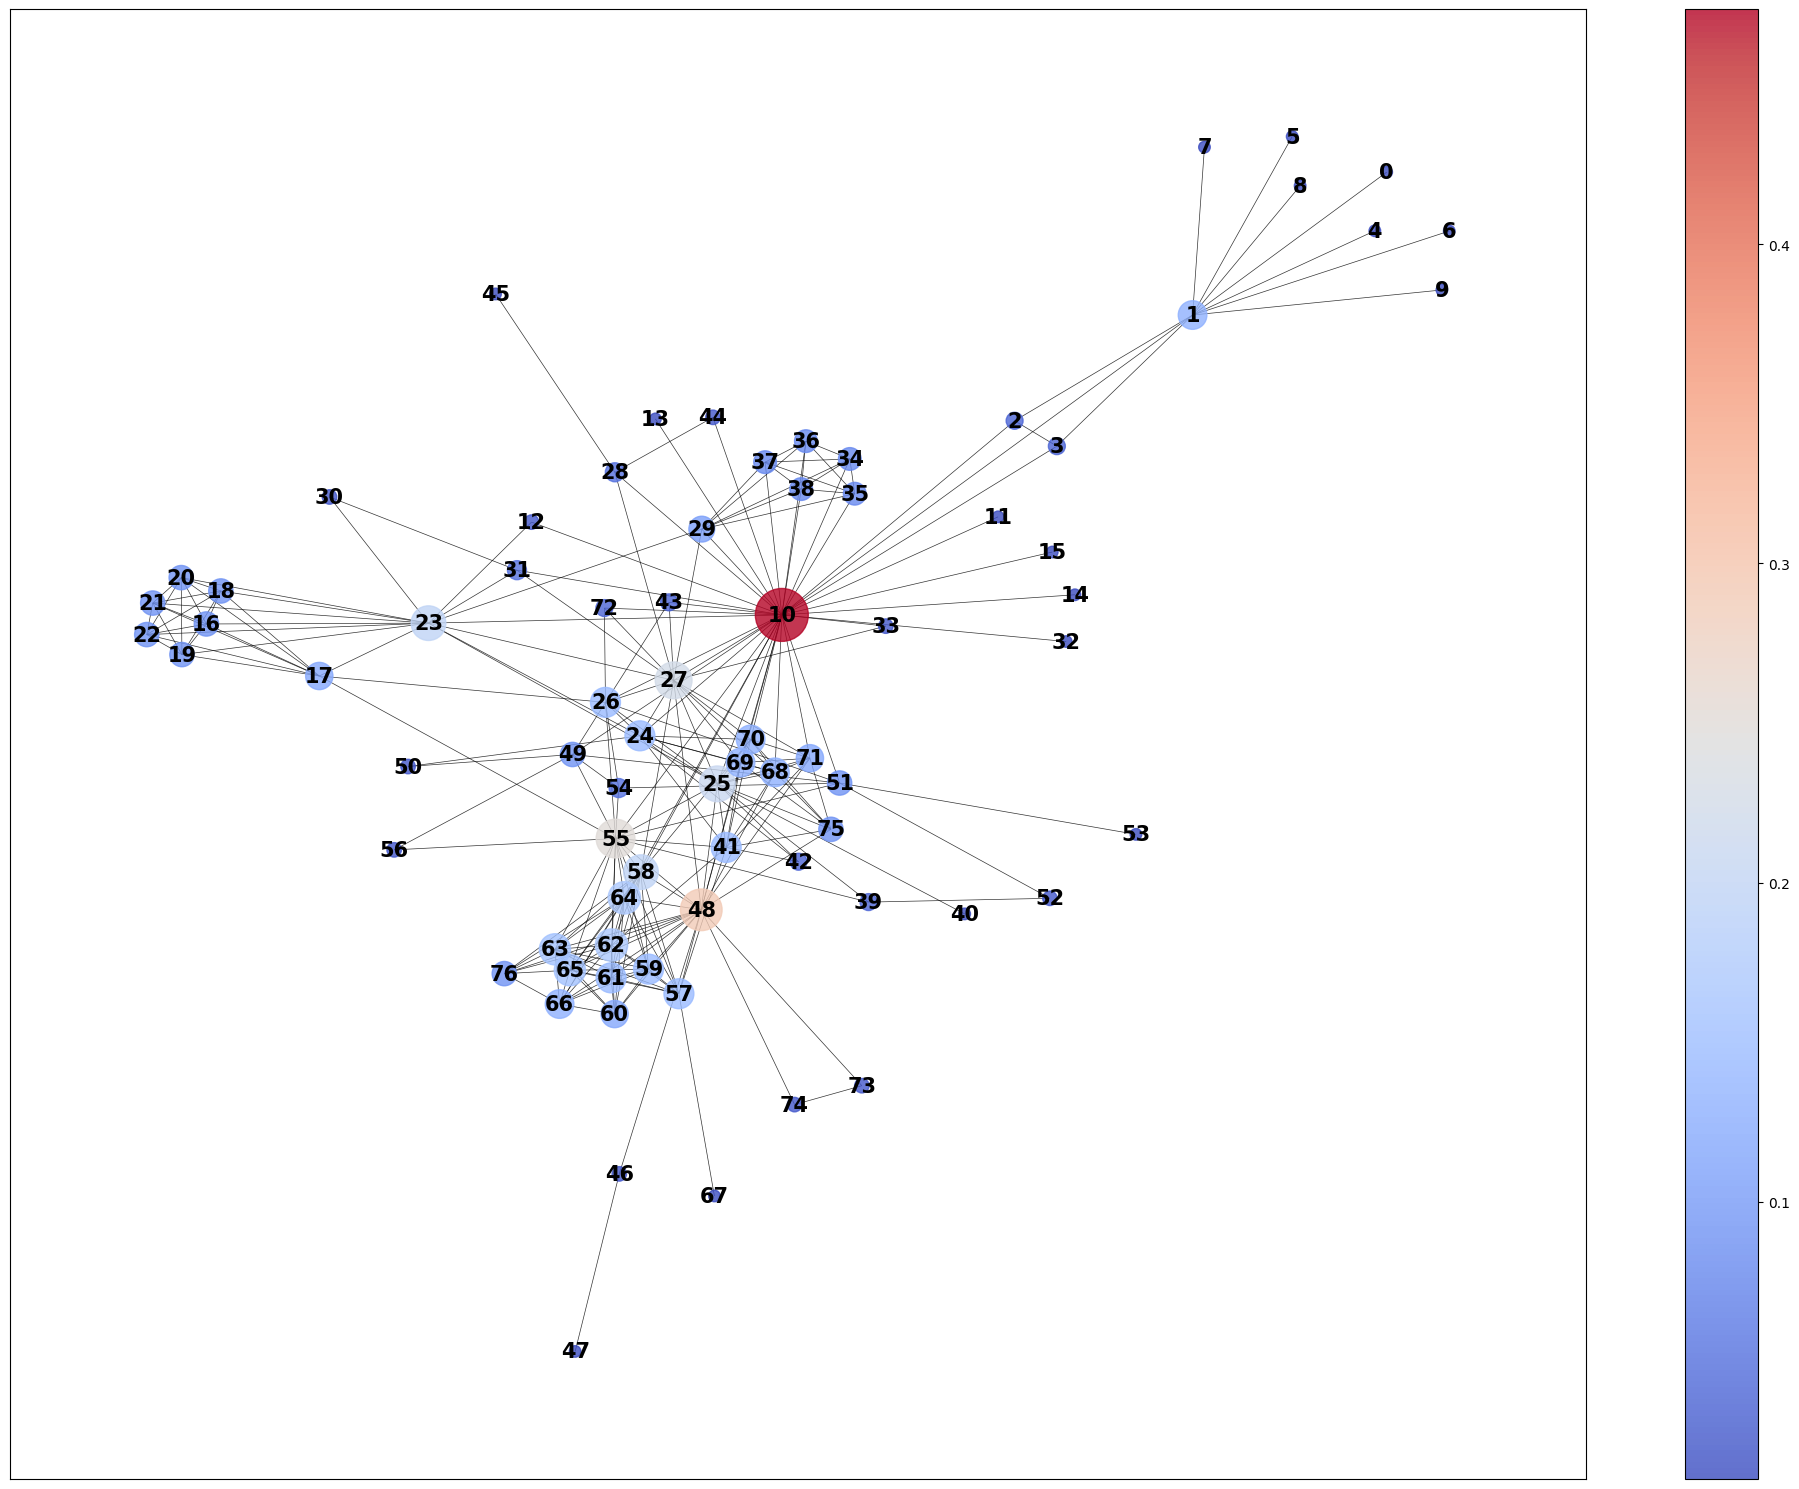
\includegraphics[width=3in]{img/les_miserables_centralidad_degree.png}
    \caption{Centralidad de grado - 'Les Miserables'}
    \label{fig:les_miserables_centralidad_deg}
\end{figure}

\begin{figure}[h]
    \centering
    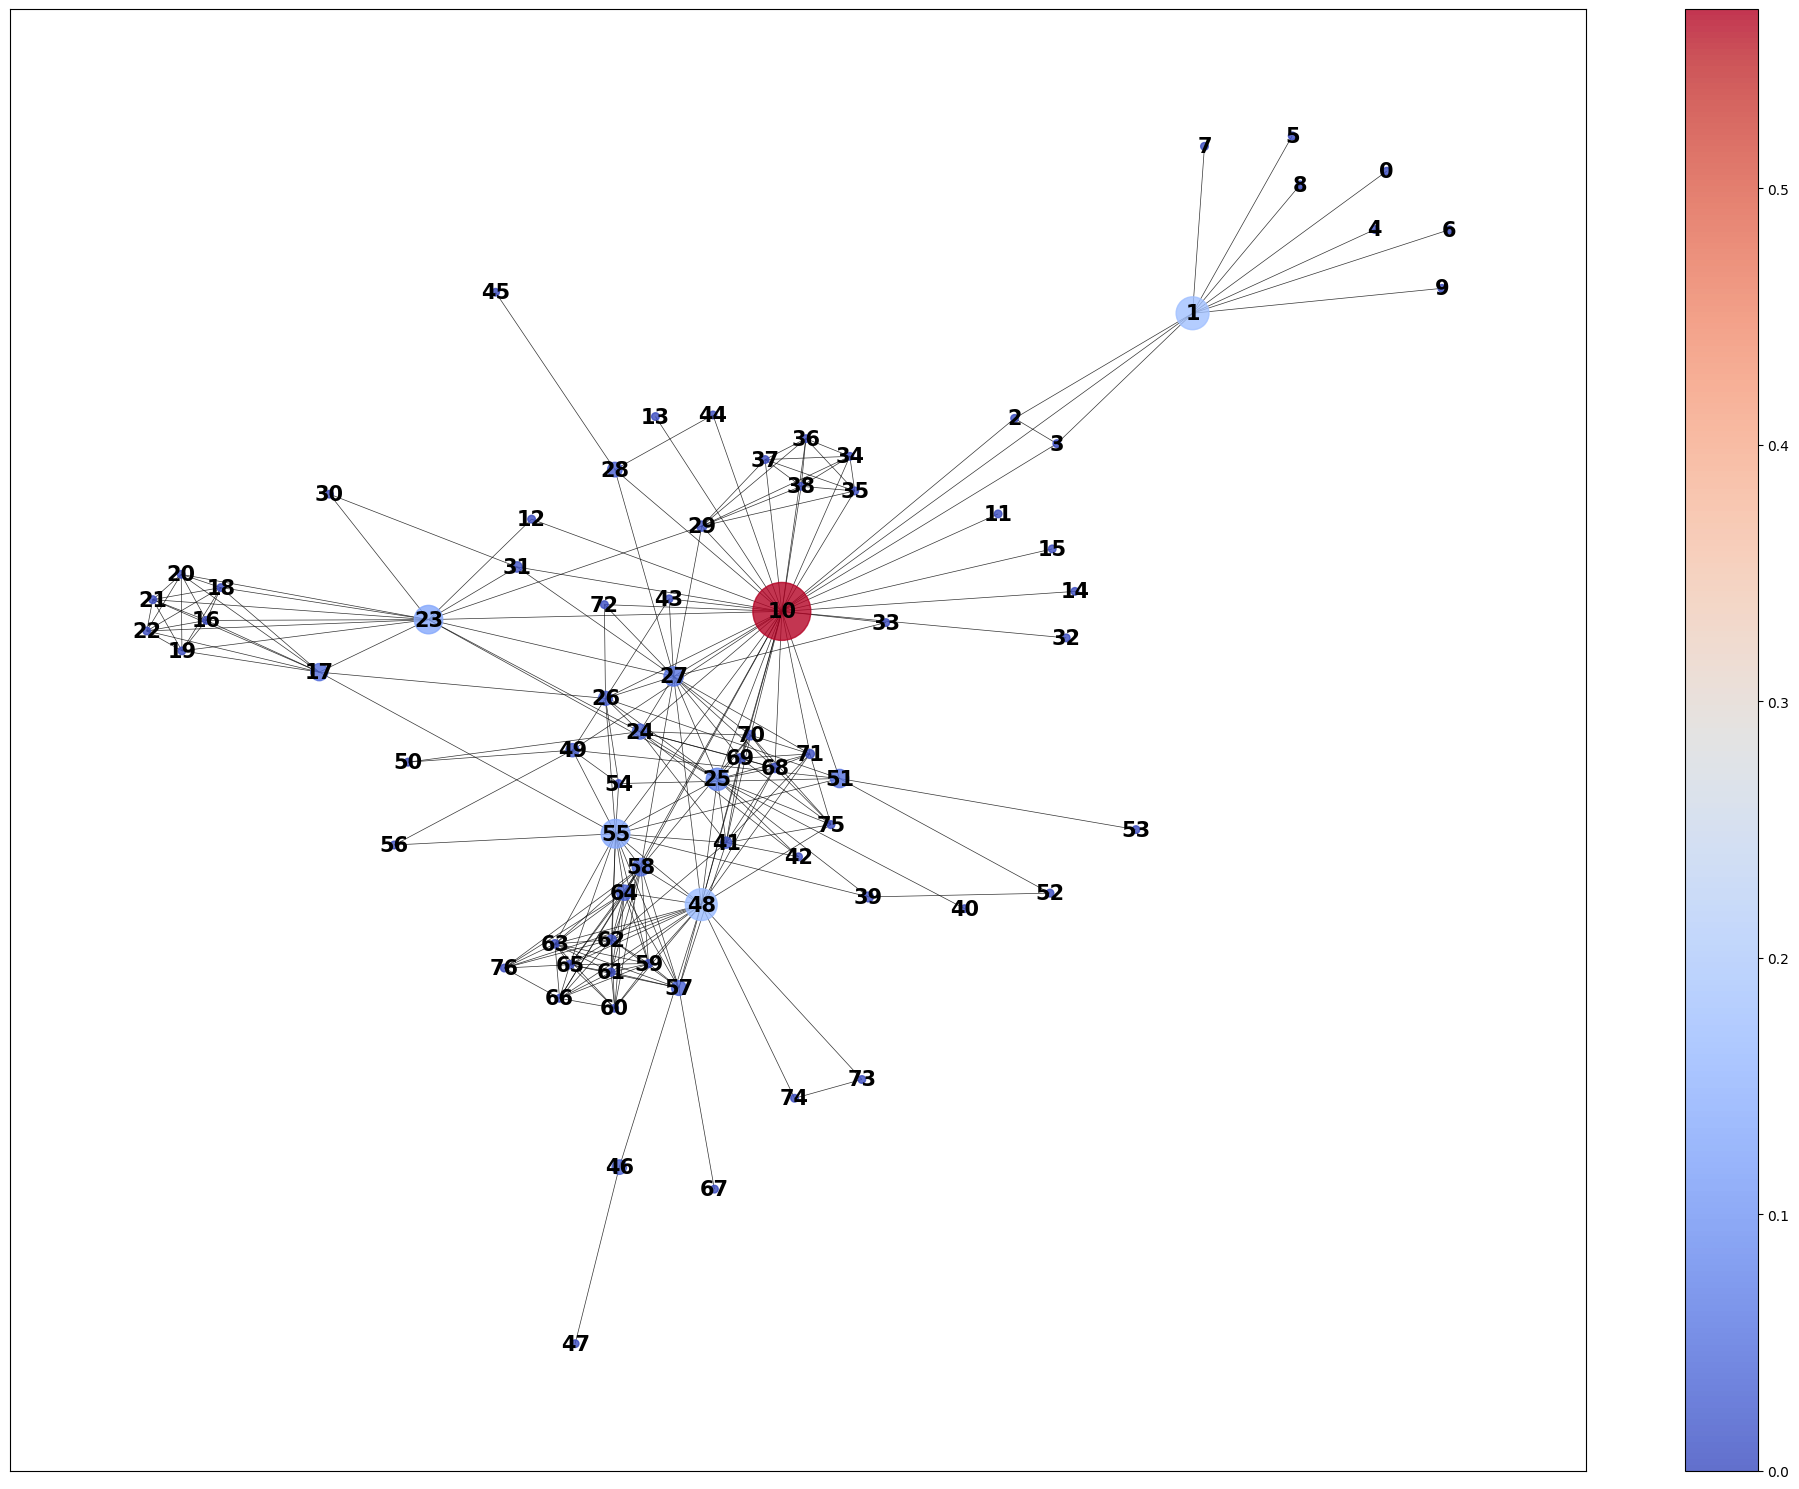
\includegraphics[width=3in]{img/les_miserables_centralidad_betweness.png}
    \caption{Centralidad de intermediación - 'Les Miserables'}
    \label{fig:les_miserables_centralidad_bet}
\end{figure}

Cuando se observa la centralidad de betweness se puede observar que que el nodo 10 mantiene su centralidad mientras que los otros cuatro disminuyen un poco. Y en este momento el nodo 1 queda emparejado a los otros cuatro. Además se puede observar en el grafo que el nodo 1 mantiene conectado a otros 7 nodos con el resto del sistema. Lo cual nos indica que su intermediación es estratégica para conectar partes del grafo.
Si lo pensamos a nivel del “negocio” en el grafo de predominancia de la centralidad se resalta la importancia de los personajes principales mientras que en el grafo que se observa la centralidad de intermediación se destacan personajes que unen escenas o personajes.



\vspace{5pt}

\subsection{Análisis de robustez}
La comparación con prototipos y el análisis de centralidad nos ofrece algunos indicios para pensar la robustez. Por un lado vemos que hay aspectos de estas redes que se asemejan al modelo de redes libres de escala y por el otro, vemos que asemejan a redes de mundo pequeño, lo cual nos lleva a hipótesis contradictorias respecto de como se van a comportar esas redes ante eventuales ataques, dirigido o aleatorios. La centralidad por su parte, nos indica una clara diferencia entre estas dos redes respecto a la intedmediación que nos permite anticipar un comportamiento distinto en relación a los ataques.
Con el fin de lograr un mejor entendimiento de las redes que permitan responder de forma más precisa esta inquietud y a la pregunta que motivó este proyecto, se procede a analizar la evolución del tamaño de la componente gigante y la eficiencia global a medida que se efectúan ataques aleatorios y estratégicos a los nodos de la red.
\begin{figure}[h]
    \centering
    \subfigure[Red de email]{%
        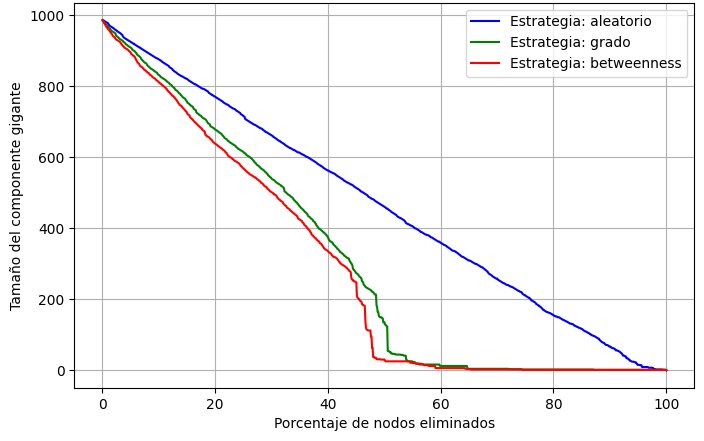
\includegraphics[width=3.5in]{img/robustez_emails_comp_gig.png}
        \label{fig:email_comp_gig}
    }
    \hfill
    \subfigure['Les Miserables']{%
        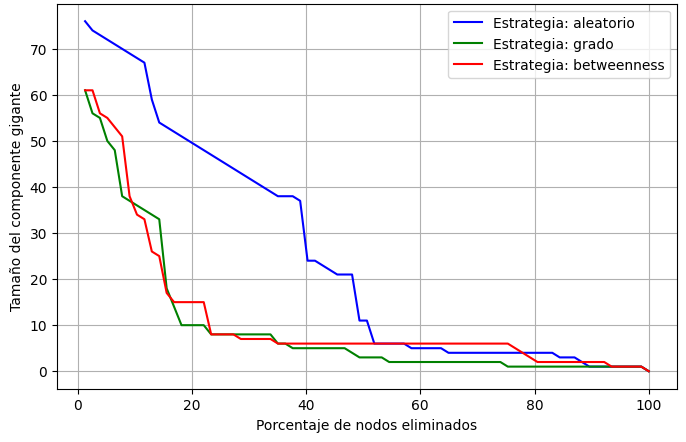
\includegraphics[width=3.5in]{img/robustez_miserables_comp_gig.png}
        \label{fig:miserables_comp_gig}
    }
    \caption{Evolución de la componente gigante en ambas redes}
    \label{fig:comp_gig_dos_redes}
\end{figure}

\begin{figure}[h]
    \centering
    \subfigure[Red de email]{%
        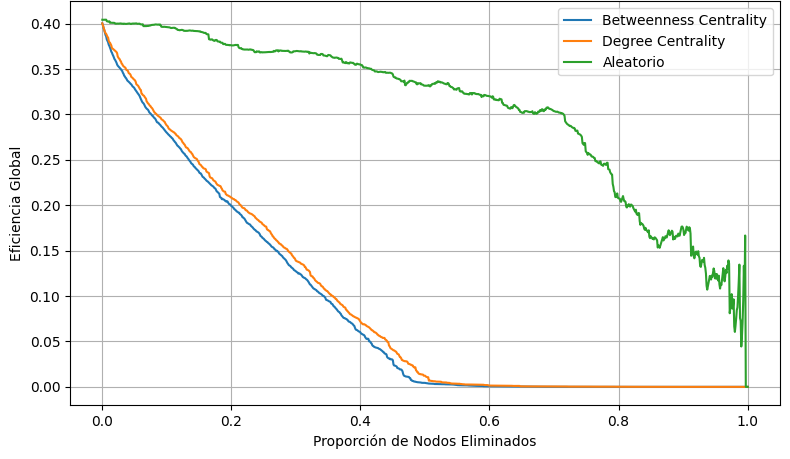
\includegraphics[width=3.5in]{img/eficienca email.png}
        \label{fig:eficiencia email}
    }
    \hfill
    \subfigure['Les Miserables']{%
        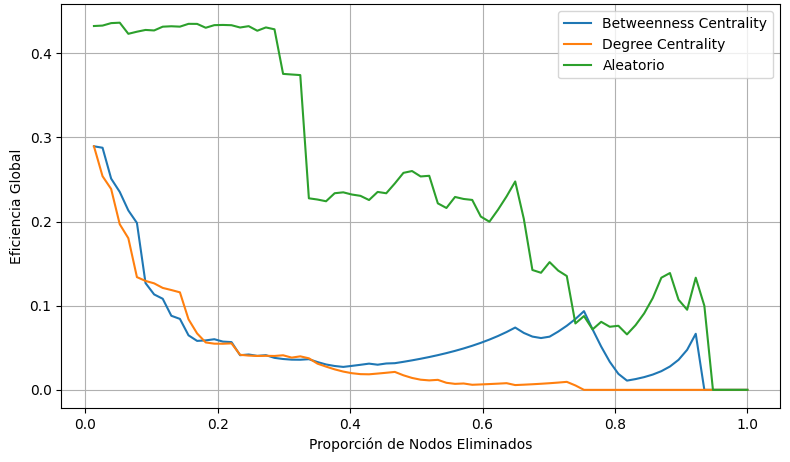
\includegraphics[width=3.5in]{img/eficiencia lesmis.png}
        \label{fig:eficiencia lesmis}
    }
    \caption{Evolución de la eficiencia global en ambas redes}
    \label{fig:comp_gig_dos_redes}
\end{figure}
%\FloatBarrier

Según se ve en los gráficos, ambas redes muestran diferencias entre sí frente a los "ataques" efectuados a las mismas. Ante a extracciones de forma aleatoria, en la red de emails se presenta una disminución lineal y estable del tamaño de la componente gigante y una caída progresiva en la eficiencia global pero de menor pendiente que el tamaño de la componente gigante, mientras que la red de 'Les Miserables' si bien presenta cierta estabilidad frente a ataques aleatorios, no es tan robusta como la red de emails, mostrando algunas caídas puntuales fuertes en el tamaño de la componente gigante y un comportamiento similar en la eficiencia global. En cuanto a extracciones hechas a nodos de alta centralidad ya sea de grado como de betweenness, se perciben diferencias notables entre ambas redes. La red de 'Les Miserables' da cuenta de una red con hubs debido a la rápida caída en el tamaño de la componente gigante (el tamaño de la componente se reduce a 1/6 de la misma con solo extraer el 20\% de los nodos de la red), acompañada de una caída de similar característica en la eficiencia global, mientras que en la red de email se observa una red más robusta que la de red de 'Les Miserables' ya que el tamaño de su componente gigante decrece en una forma gradual y con una sola caída abrupta, lo que da cuenta de una posible red de mundos pequeños en los que se forman comunidades entre las personas que se comunican vía mail. La red de 'Les Miserables' al contar con protagonistas que se relacionan con la mayoría de los personajes a lo largo de la historia provoca que sin su presencia en la red la misma sea mucho menos conexa. En cuanto a la eficiencia global las caídas son similares a la producida en la componente gigante para cada red lo cual reafirma la idea de una red de mundo pequeño para los email (lo cual luego se analizará en la sección de comunidades) y una red más similar a una red libre de escala para 'Les Miserables'.

\vspace{5pt}

\subsection{Comunidades}

La detección de comunidades arrojó resultados esperables. Mientras que la red de 'Les Miserables' dio buenos niveles de modularidad y un número de clusters razonable con el tamaño de la red independientemente del algoritmo utilizado, la red de Emails EU arrojó valores más bajos de modularidad y una gran disparidad de resultados dependiendo del algoritmo utilizado (Louvain y Girvan-Newman)

\begin{figure}[h]
    \centering
    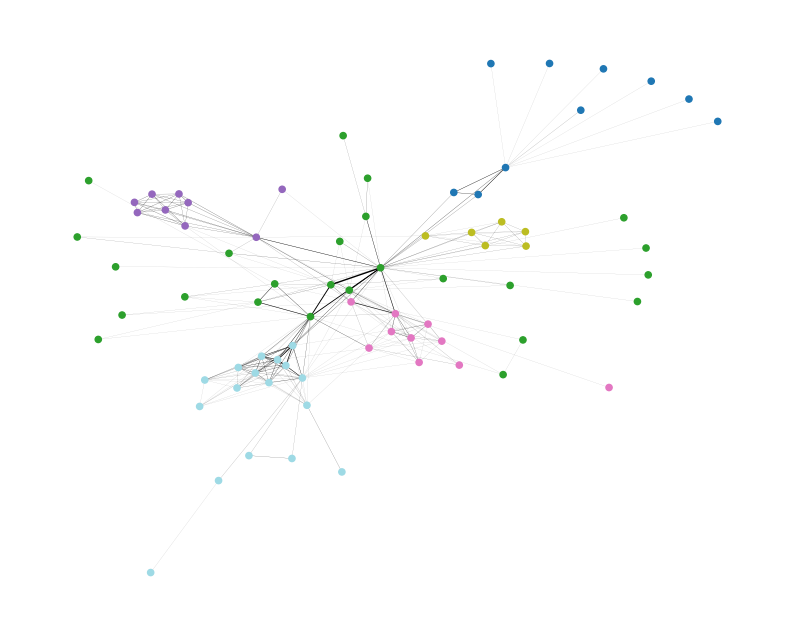
\includegraphics[width=\linewidth]{img/lesmisLouvainGraph.png}
    \caption{Red de 'Les Miserables' coloreada por clusters}
    \label{fig:lesmis_louvain}
\end{figure}

Como se puede ver en la figura \ref{fig:lesmis_louvain} las comunidades son muy claras y con bajo nivel de superposición, lo cual coincide con el valor de modularidad obtenido 0.5654. Esta claridad tal vez esté relacionada al hecho de ser una red artificial creada a partir de la copresencia de personajes de una novela clásica, es probable que estas comunidades sean similares a los grupos identificables en la novela (los revolucionarios, los delincuentes, los religiosos, etc.) 

\begin{figure}[h]
    \centering
    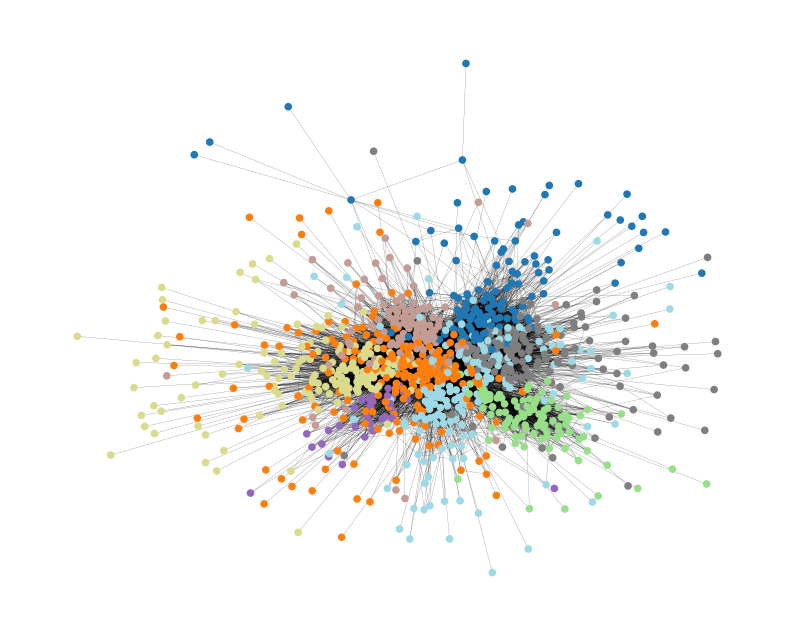
\includegraphics[width=\linewidth]{img/emailLouvainGraph.png}
    \caption{Red de Emails coloreada por clusters}
    \label{fig:emails_louvain}
\end{figure}

Como podemos ver en la imagen \ref{fig:emails_louvain} se detectaron comunidades con una modularidad moderadamente alta, en el grafo pueden distinguirse las comunidades agrupadas por color con claridad, pero a la vez se puede observar un cierto nivel de superposición. La modularidad obtenida en la partición óptima fue de 0.4160.

En los Emails solo vamos a considerar las comunidades detectadas mediante el algoritmo de Louvain, ya que Girvan-Newman arrojó valores de modularidad muy bajos.

Retomando el análisis de robustez podemos ver cómo la modularidad de estas redes puede funcionar como complemento. La red 'Les Miserable' con su alta modularidad y clara estructura comunitaria es a la vez vulnerable a los ataques dirigidos, lo cual indica que unos pocos nodos (con alto grado de intermediación) son quienes sostienen esta estructura comunitaria y que su eliminación descompone la conectividad de la red y la interacción entre sus comunidades. 
La red de emails en cambio, muestra una estructura más integrada, aun con una modularidad considerablemente fuerte, pero con cierto nivel de superposición entre comunidades, esto también la hace más resistente a ataques dirigidos, ya que al tener un alto nivel de redundancia dentro de las comunidades no depende tan fuertemente de los nodos con alta intermediación.

A la hora de comparar los datos de departamentos con las particiones de modularidad comenzamos utilizando el Adjusted Random Score, que dio un resultado relativamente bajo de 0.3250. Al notar la importante diferencia de escala entre las particiones que estábamos comparando, 42 departamentos contra 8 comunidades, decidimos complementar con otros métodos.
La primera métrica complementaria utilizada fue Normalized Mutual Information, que al estar normalizada por entropía evita penalizar las diferencias de granularidad. Con esta métrica se obtuvo un resultado considerablemente mayor 0.5813. Lo cual indica niveles de similaridad mayores, aun cuando la cantidad de departamentos y comunidades sea disímil.
Siguiendo esta idea utilizamos una tabla de contingencia acompañada por un heatmap para evaluar la asociación entre departamentos y comunidades.

\begin{figure}[!h]
    \centering
    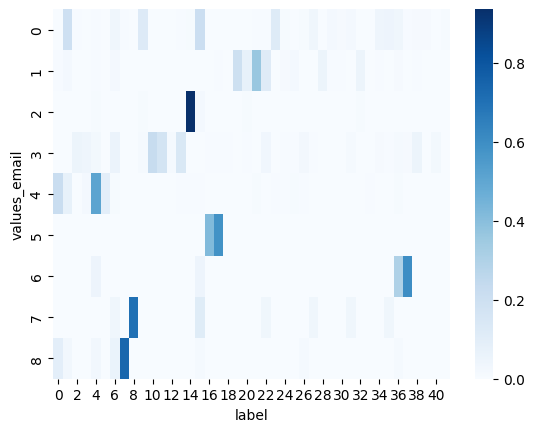
\includegraphics[width=\linewidth]{img/comu_contingencia_deptcom.png}
    \caption{Heatmap entre comunidades detectadas por el algoritmo Louvain y las etiquetas de departamentos de la red Emails EU}
    \label{fig:enter-label}
\end{figure}
\FloatBarrier
Como se puede ver en la figura, hay algunas asociaciones importantes, al menos 6 de las 8 comunidades que tienen una asociación fuerte con al menos un departamento. Esto estaría indicando que más allá de las diferencias de modularidad hay una asociación importante entre la mayoría de las comunidades y algunos de los departamentos. Si bien es una temática interesante para profundizar, entendemos que excede el alcance del presente documento; queda entonces como pregunta para indagaciones futuras.

\vspace{15pt}

\section{\textbf{Conclusiones}}

\vspace{10pt}
En la comparación con los modelos prototípicos, observamos que ninguna de las redes analizadas se alinea completamente con un único prototipo. Si bien la distribución de grado se asemeja a la de las redes libres de escala, el coeficiente de clustering se acerca más al de las redes de mundo pequeño.

El análisis de centralidad reveló similitudes en la centralidad de grado entre ambas redes, pero diferencias notables en la centralidad de intermediación. Esta diferencia impacta significativamente la detección de comunidades. En la red de 'Les Miserables', la alta modularidad obtenida (resultados de Louvain y Girvan-Newman) está fuertemente influenciada por un grupo de nodos con alta intermediación. En contraste, la red de Emails EU, con valores de intermediación relativamente más bajos, presenta una modularidad menor (según Louvain y mucho menor según Girvan-Newman).

El análisis de robustez complementa estos hallazgos, revelando diferencias clave entre las redes. En general, la red de Emails EU es más resiliente que la de 'Les Miserables', especialmente frente a fallos o ataques dirigidos a nodos clave.

Esta resiliencia de la red de Emails EU sugiere una estructura más redundante y menos dependiente de hubs específicos. Este patrón podría reflejar la presencia de múltiples rutas de comunicación entre grupos, característica de redes con comunidades bien definidas. Sin embargo, aunque la modularidad óptima mediante Louvain es considerablemente alta (0,4160), la baja modularidad obtenida con Girvan-Newman \textless~0.1 plantea interrogantes sobre la solidez de esta estructura comunitaria. La alta resiliencia sugiere que, aunque la estructura comunitaria no sea tan clara, la red cuenta con rutas alternativas para mantener la conectividad.

La alta modularidad de la red de 'Les Miserables', junto con el alto grado de intermediación de algunos actores clave (hubs), explica su vulnerabilidad frente a ataques dirigidos. Este patrón puede estar influenciado por el tamaño relativamente pequeño de la red (n=77).

En resumen, aunque ambas redes involucran actores humanos, su estructura responde a lógicas distintas. La red de 'Les Miserables' representa una narrativa centrada en personajes protagonistas, cuya presencia es clave para conectar el grafo. Esta estructura, fruto de la imaginación del autor, la hace vulnerable a la eliminación de esos nodos clave. En cambio, la red de Emails EU refleja un entorno organizacional real donde, si bien existen nodos relevantes, la información puede seguir fluyendo —aunque menos eficientemente— incluso si estos nodos se eliminan, gracias a la interconexión y el solapamiento entre grupos.

Podemos concluir que el carácter idealizado de la red de 'Les Miserables', fruto de un relato que busca contar una historia de modo atractivo y comprensible, influye en el peso de los actores clave (hubs), transformándola en una red frágil ante ataques dirigidos. En contraste, el carácter realista de la red de Emails EU, resultado de la interacción efectiva entre miembros de una organización, lejana a cualquier idealización, la hace más resiliente. Mientras que la historia detrás de 'Les Miserables' es coherente, bien organizada y atractiva, la historia detrás de los Emails EU resulta compleja, desordenada, difícil de entender y presumiblemente poco atractiva, aunque más resiliente.

Esto nos deja algunos interrogantes que invitan a un debate posterior. ¿Es esta resiliencia común a las redes de interacción humana? ¿Qué contraejemplos podemos encontrar en la literatura sobre redes? ¿Qué aspectos inciden en la conformación de hubs en este tipo de redes? 

\begin{thebibliography}{00}
\bibitem{mouschoutzi2024}
M.~Mouschoutzi, ``Les Misérables Social Network Analysis using Marimo notebooks and the NetworkX Python library,'' \emph{Towards Data Science}, Mar. 2024. [Online]. 
Available: \href{https://towardsdatascience.com/les-miserables-social-network-analysisusing-marimo-notebooks-and-the-networkx-python-library-%EF%B8%8F-%EF%B8%8F-3f433216412f/}{towardsdatascience.com}


\bibitem{nr} 
R.~A. Rossi and N.~K. Ahmed, ``The Network Data Repository with Interactive Graph Analytics and Visualization,'' in \emph{Proc. AAAI}, 2015. [Online]. Available: \url{https://networkrepository.com}

\bibitem{barabasi2016}
A.-L. Barabási, ``Network Science,'' Cambridge University Press, 2016. [Online]. Available: \url{https://networksciencebook.com}

\bibitem{networkx2008}
Hagberg, A. A., Swart, P. J., \& S Chult, D.. Exploring network structure, dynamics, and function using NetworkX. In Proceedings of the 7th Python in Science Conference (SciPy2008), 2008. [Online]. La versión utilizada es 3.4.1, la documentación está dispobible en: \url{https://networkx.org/documentation/networkx-3.4.1/reference/index.html}

\end{thebibliography}
\vspace{12pt}

\end{document}